\documentclass[12pt]{article}
\usepackage{graphicx}

%%%%%%%%%%%%%%%%%%%%%%%%%%%%%%%%%%%%%%%%%%%%%%%%%%%%%%%%%%%%%%%%%%%%
% basic data for the eprint:
%%%%%%%%%%%%%%%%%%%%%%%%%%%%%%%%%%%%%%%%%%%%%%%%%%%%%%%%%%%%%%%%%%%%

\textwidth=6.0in  \textheight=8.25in

%%  Adjust these for your printer:
\leftmargin=-0.3in   \topmargin=-0.20in

%% preprint number data:
\newcommand\pubnumber{}%SNSN-323-63}
\newcommand\pubdate{\today}

%%  address and funding acknowledgement data:
\def\institute{Centre for Cosmology, Particle Physics and Phenomenology\\
Universit\'e catholique de Louvain, B-1348 Louvain-la-Neuve, BELGIUM}
\def\support{\footnote{Work supported by Fonds de la Recherche Scientifique (FNRS), Belgium.}}

%%%%%%%%%%%%%%%%%%%%%%%%%%%%%%%%%%%%%%%%%%%%%%%%%%%%%%%%%%%%%%%%%%%%%%%%%%%%
%   document style macros
%%%%%%%%%%%%%%%%%%%%%%%%%%%%%%%%%%%%%%%%%%%%%%%%%%%%%%%%%%%%%%%%%%%%%%%%%%%%
\def\Title#1{\begin{center} {\Large #1 } \end{center}}
\def\Author#1{\begin{center}{ \sc #1} \end{center}}
\def\Address#1{\begin{center}{ \it #1} \end{center}}
\def\andauth{\begin{center}{and} \end{center}}
\def\submit#1{\begin{center}Submitted to {\sl #1} \end{center}}
\newcommand\pubblock{\rightline{\begin{tabular}{l} \pubnumber\\
         \pubdate  \end{tabular}}}
\newenvironment{Abstract}{\begin{quotation}  }{\end{quotation}}
\newenvironment{Presented}{\begin{quotation} \begin{center} 
             PRESENTED AT\end{center}\bigskip 
      \begin{center}\begin{large}}{\end{large}\end{center} \end{quotation}}
\def\Acknowledgements{\bigskip  \bigskip \begin{center} \begin{large}
             \bf ACKNOWLEDGEMENTS \end{large}\end{center}}
%%%%%%%%%%%%%%%%%%%%%%%%%%%%%%%%%%%%%%%%%%%%%%%%%%%%%%%%%%%%%%%%%%%%%%%%%%%%
%  personal abbreviations and macros
%    the following package contains macros used in this document:
\input econfmacros.tex
\input mycommands.tex
%%%%%%%%%%%%%%%%%%%%%%%%%%%%%%%%%%%%%%%%%%%%%%%%%%%%%%%%%%%%%%%%%%%%%%%%%%%

\begin{document}
\begin{titlepage}
\pubblock

\vfill
\Title{Measurement of the differential cross section for t-channel single-top-quark production at 13 TeV}
\vfill
\Author{ Matthias Komm\support, on behalf of the CMS collaboration}
\Address{\institute}
\vfill
\begin{Abstract}
The production of single top quarks is a cornerstone in understanding the nature of the heaviest known elementary particle and its involvement in electroweak interactions. An early differential cross section measurement of t-channel single-top-quark production is presented. Collision data at a center-of-mass energy of $13~\mathrm{TeV}$ collected in 2015 were analyzed, corresponding to $2.3~\mathrm{fb}^{-1}$. The amount of signal events as a function of the top quark transverse momentum and rapidity is estimated by multiple fits using a multivariate discriminant. The results are unfolded to parton level and compared to predictions by various Monte-Carlo generators.
\end{Abstract}
\vfill
\begin{Presented}
$9^{th}$ International Workshop on Top Quark Physics\\
Olomouc, Czech Republic,  September 19--23, 2016
\end{Presented}
\vfill
\end{titlepage}
\def\thefootnote{\fnsymbol{footnote}}
\setcounter{footnote}{0}
%

\section{Introduction}

Cross section measurements of single top quark production allow to study electroweak interactions involving heavy quarks. For example, precise inclusive cross section measurements can yield model-independent limits on the CKM matrix element, $\mathrm{V}_\mathrm{tb}$, whereas differential measurements can test theoretical calculations and predictions by generators in great detail.

In this note, a first differential cross section of t-channel single-top-quark production as a function of the top quark \pt and rapidity, $y=\frac{1}{2}\ln[(E+p_{z})/(E-p_{z})]$, is presented, using the first pp collision data recorded by the CMS experiment in 2015 at $\sqrt{s}=13~\mathrm{TeV}$ corresponding to $2.3~\mathrm{fb}^{-1}$. It is based on Ref.~\cite{TOP-16-004}.

\section{Event selection}

The measurement focuses on single top quarks decaying to a b jet, a muon, and a neutrino. The t-channel production signature consists furthermore of a light, spectator quark~(u/d/s) which is characteristically scattered into the forward detector region. Muon candidates are required to be well-isolated with a transverse momentum of $\pt>22~\mathrm{GeV}$ within a pseudorapidity range of $|\eta|<2.4$. Jets with $\pt>40~\mathrm{GeV}$ are selected within $|\eta|<4.7$. A b-tagging algorithm is employed for jets within $|\eta|<2.4$ based on a multivariate discriminant to identify b jets from top quark decays. A selection on the transverse W boson mass of $\mtw>50~\mathrm{GeV}$ is applied discriminate against multijet events. In addition to the signal region~(2~jets, 1~b-tag), events from two control regions containing 3~jets with 1~or 2~b-tags are considered. These are enriched in \ttbar events which is the main background of this measurement.


\section{Signal extraction}

A neutrino candidate is found by solving for the unknown $p_{z}^{\nu}$ momentum under a W boson mass constraint, $m_{W}^{2}=(p_{\mu}+p_{\nu})^{2}$. The 4-momentum of a top quark candidate can then be reconstructed from the reconstructed decay products.

To extract the signal yield as a function of the reconstructed top quark \pt and $|y|$, multiple, exclusive maximum likelihood fits are performed. The fits utilize an extended likelihood using the $\mtw$ shape for events with $\mtw<50~\mathrm{GeV}$ and the shape of a Boosted Decision Tree~(BDT) discriminant otherwise. The BDT is trained to discriminate signal against \ttbar and \wjets events by exploiting the following event observables: $\mtop$, $|\eta_\mathrm{light~jet}|$, $\Delta R(\mathrm{b\mbox{-}jet,~light~jet})$, $|\Delta\eta(\mathrm{b\mbox{-}jet,\mu})|$, and \mtw. The low $\mtw$ region is particularly sensitive to the multijet contribution whose shape is estimated from data using a sideband with inverted muon isolation. Figure~\ref{fig:mtwbdt} shows the $\mtw$ and BDT distributions after scaling the predictions to the inclusive fit result. A good agreement is observed.

\begin{figure}[th]
\begin{center}
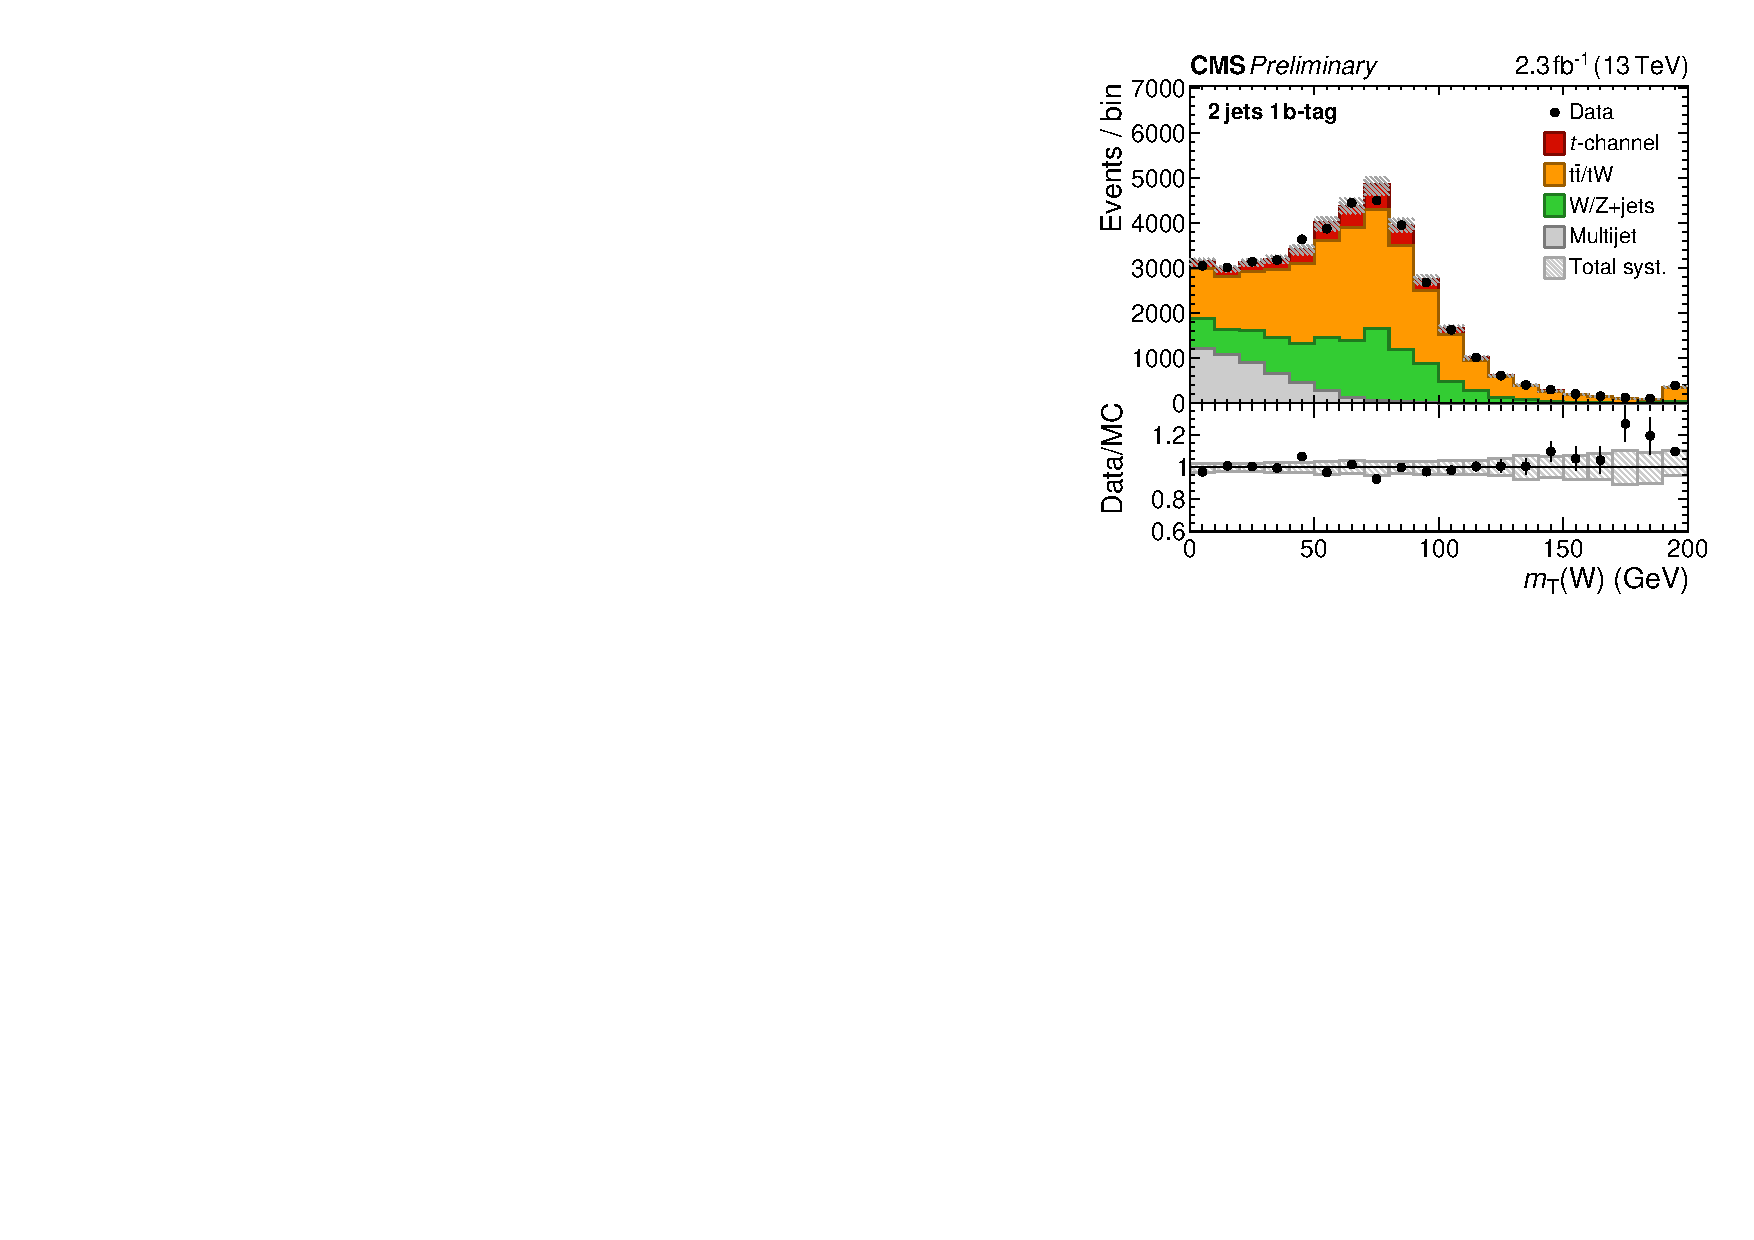
\includegraphics[width=0.45\textwidth]{figures/fit/reco_mtw.pdf}\hspace{0.05\textwidth}
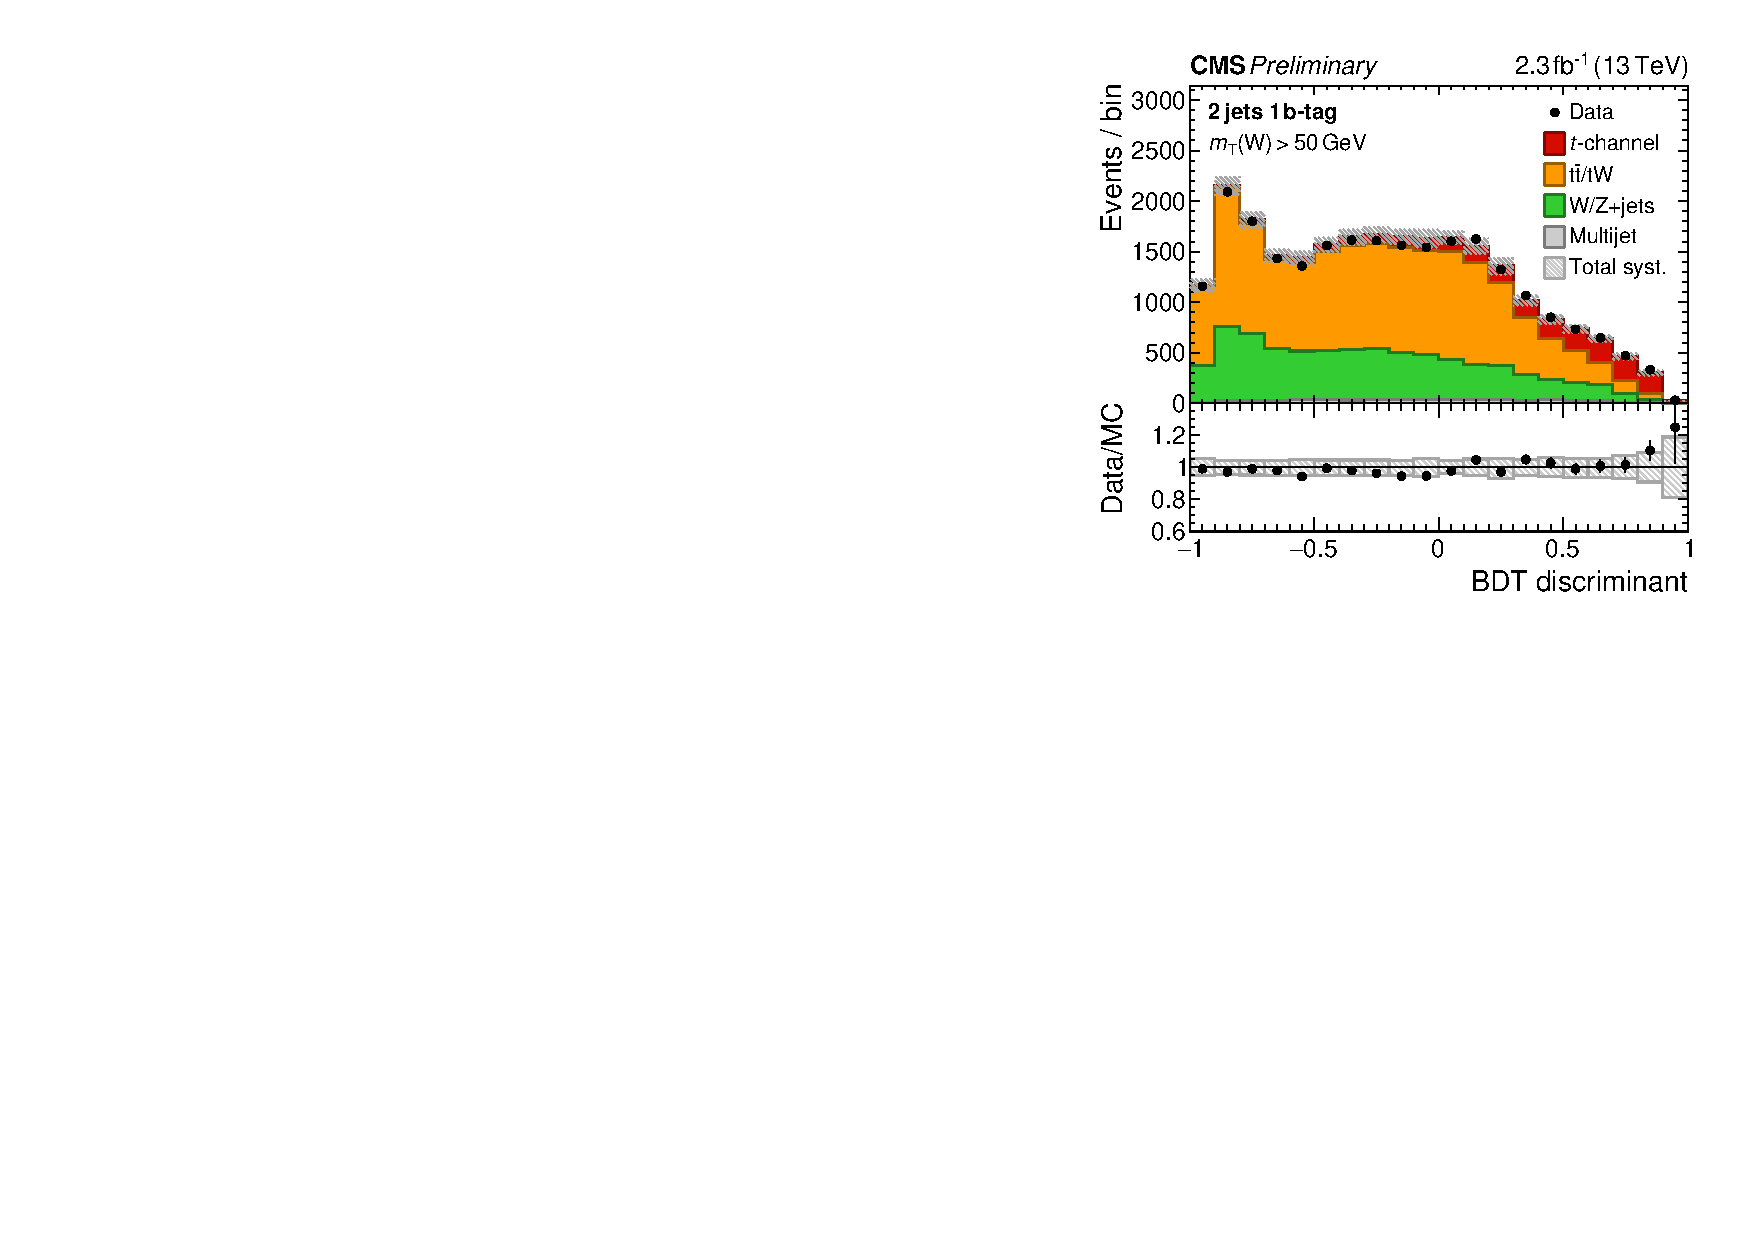
\includegraphics[width=0.45\textwidth]{figures/fit/reco_BDT.pdf}
\end{center}

\caption{\label{fig:mtwbdt}Distributions of (left)~the transverse W boson mass and (right)~the BDT discriminant after requiring $\mtw>50~\mathrm{GeV}$.}
\end{figure}

The distributions of the top quark \pt and $|y|$ at reconstruction level normalized to the inclusive fit result are shown in Fig.~\ref{fig:recotop} in a signal-enhanced phase space defined by $\mtw>50~\mathrm{GeV}$ and $\mathrm{BDT}>0.6$. The distribution of the top quark rapidity agrees well with the prediction. However, a slight 

\begin{figure}[th]
\begin{center}
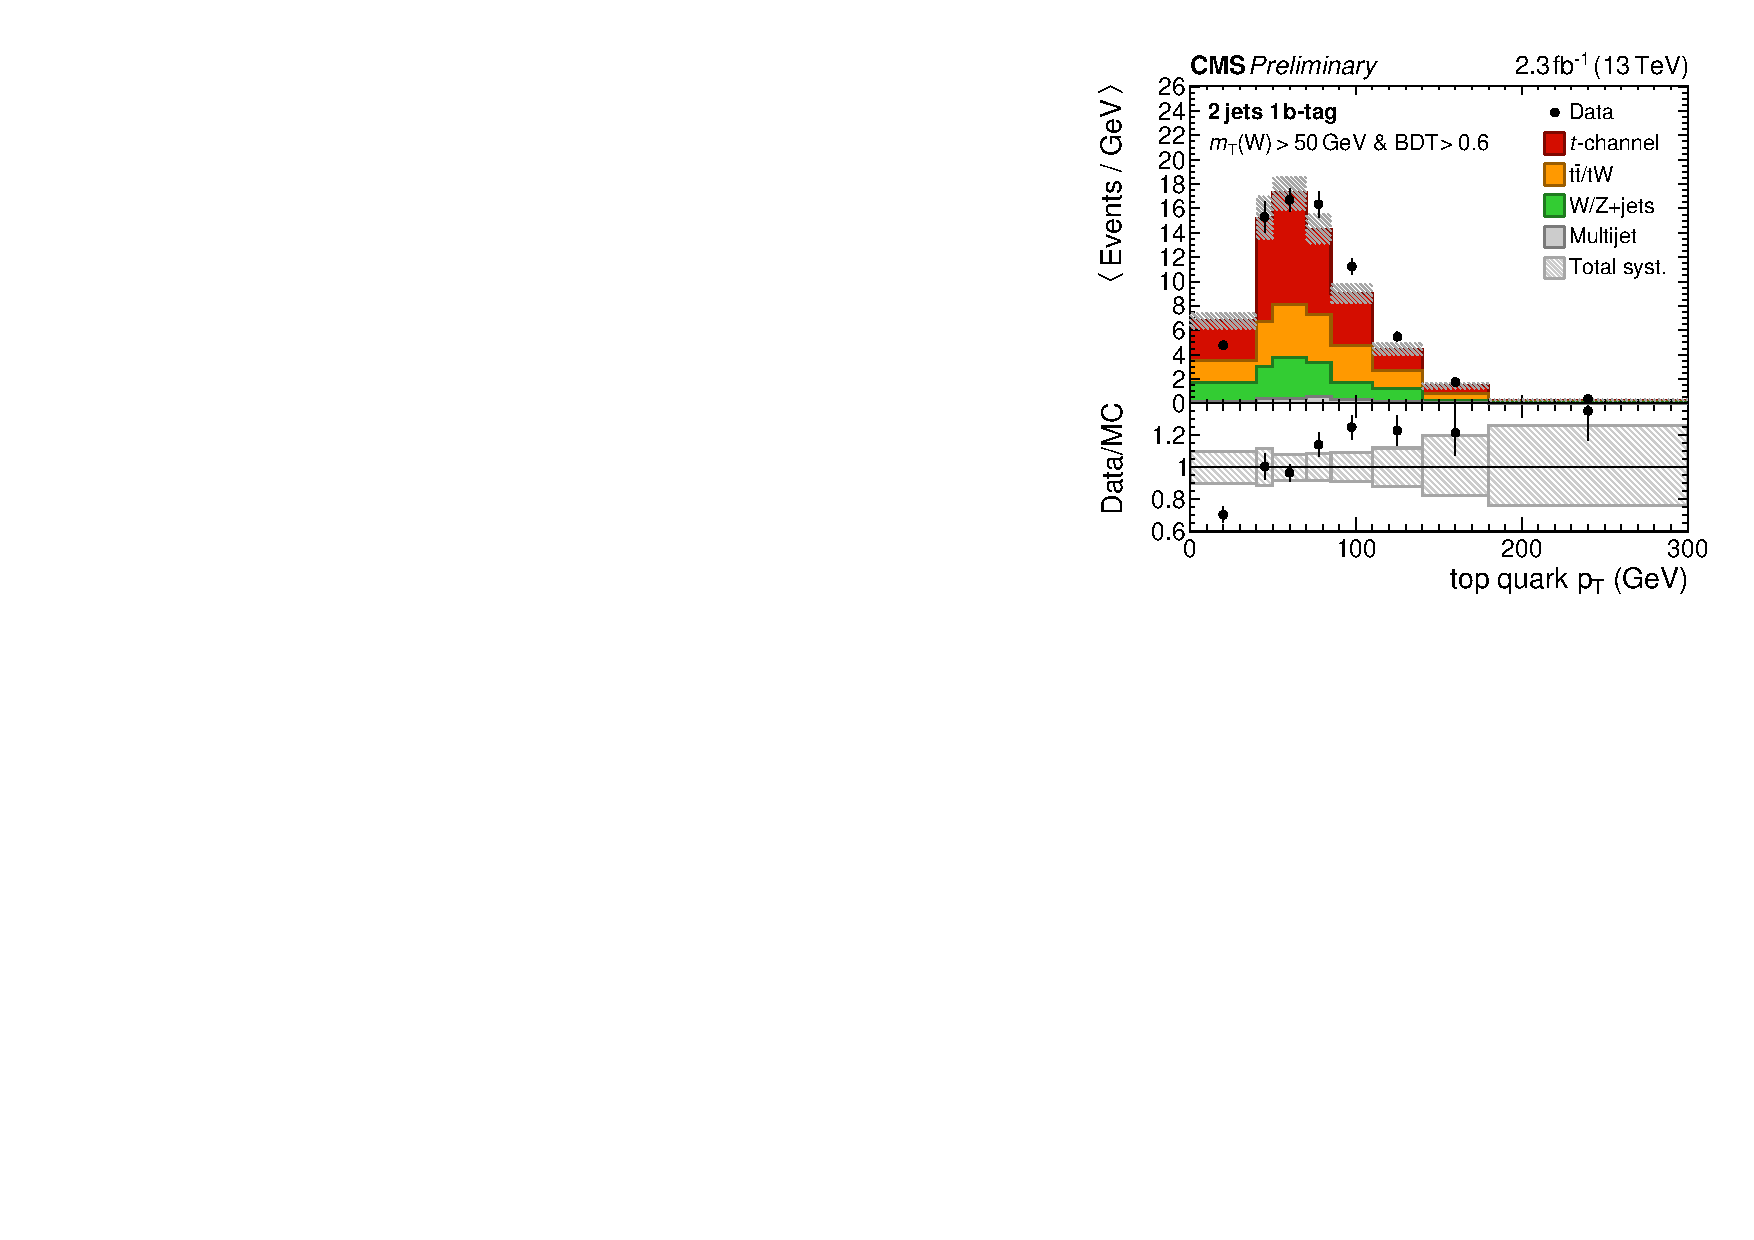
\includegraphics[width=0.45\textwidth]{figures/unfolding/reco_toppt_bdt.pdf}\hspace{0.05\textwidth}
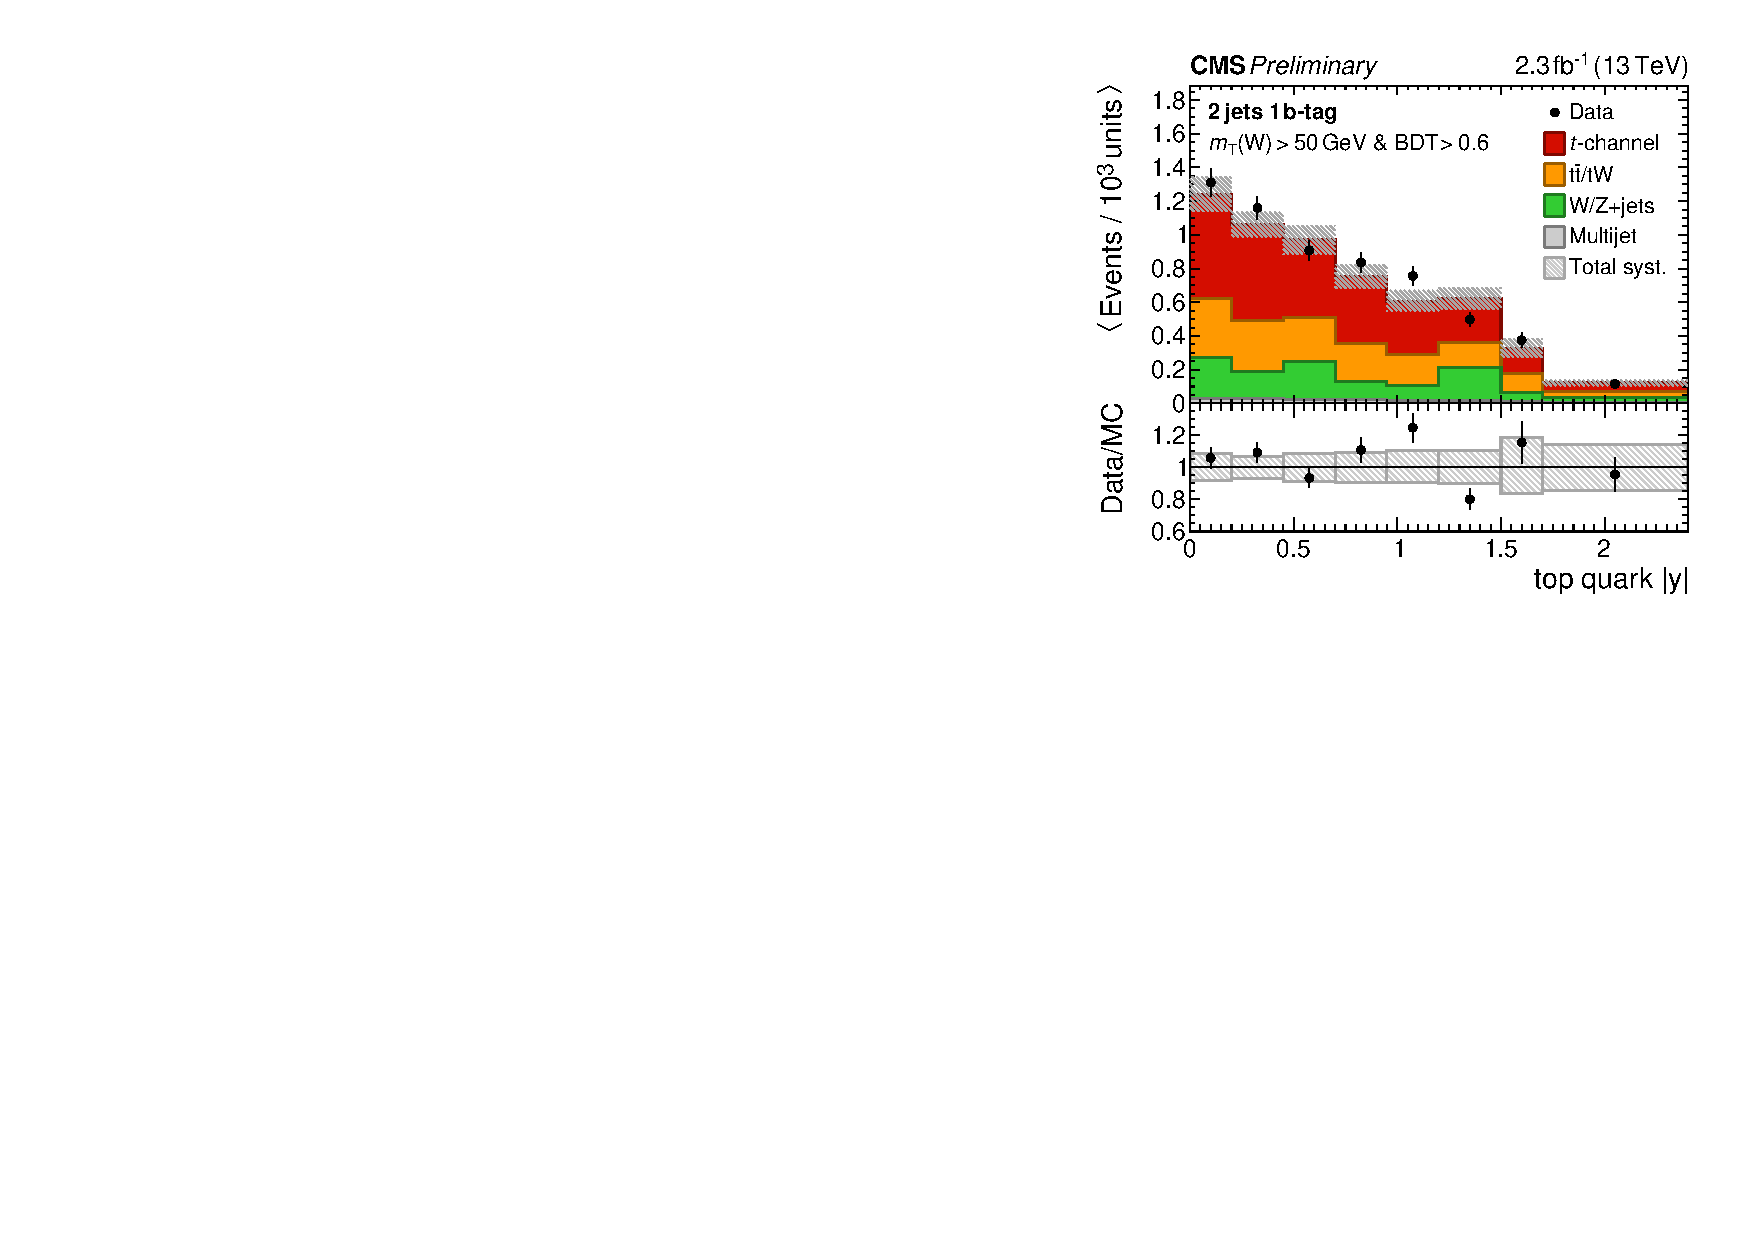
\includegraphics[width=0.45\textwidth]{figures/unfolding/reco_topy_bdt.pdf}
\end{center}

\caption{\label{fig:recotop}Distributions of the top quark (left)~transverse momentum and (right)~rapidity in a signal-enhanced phase space defined by $\mtw>50~\mathrm{GeV}$ and $\mathrm{BDT}>0.6$. Predictions are normalized to the inclusive fit result.}
\end{figure}

To infer the corresponding parton-level differential cross sections, the exclusive fit results are passed to an unfolding procedure. Regularized unfolding based on the curvature of the unfolded spectrum as implemented in the \tunfold package~\cite{tunfold} is used. 

The measurement is affected by various sources of systematics. 



\section{Results}

\begin{figure}[th]
\begin{center}
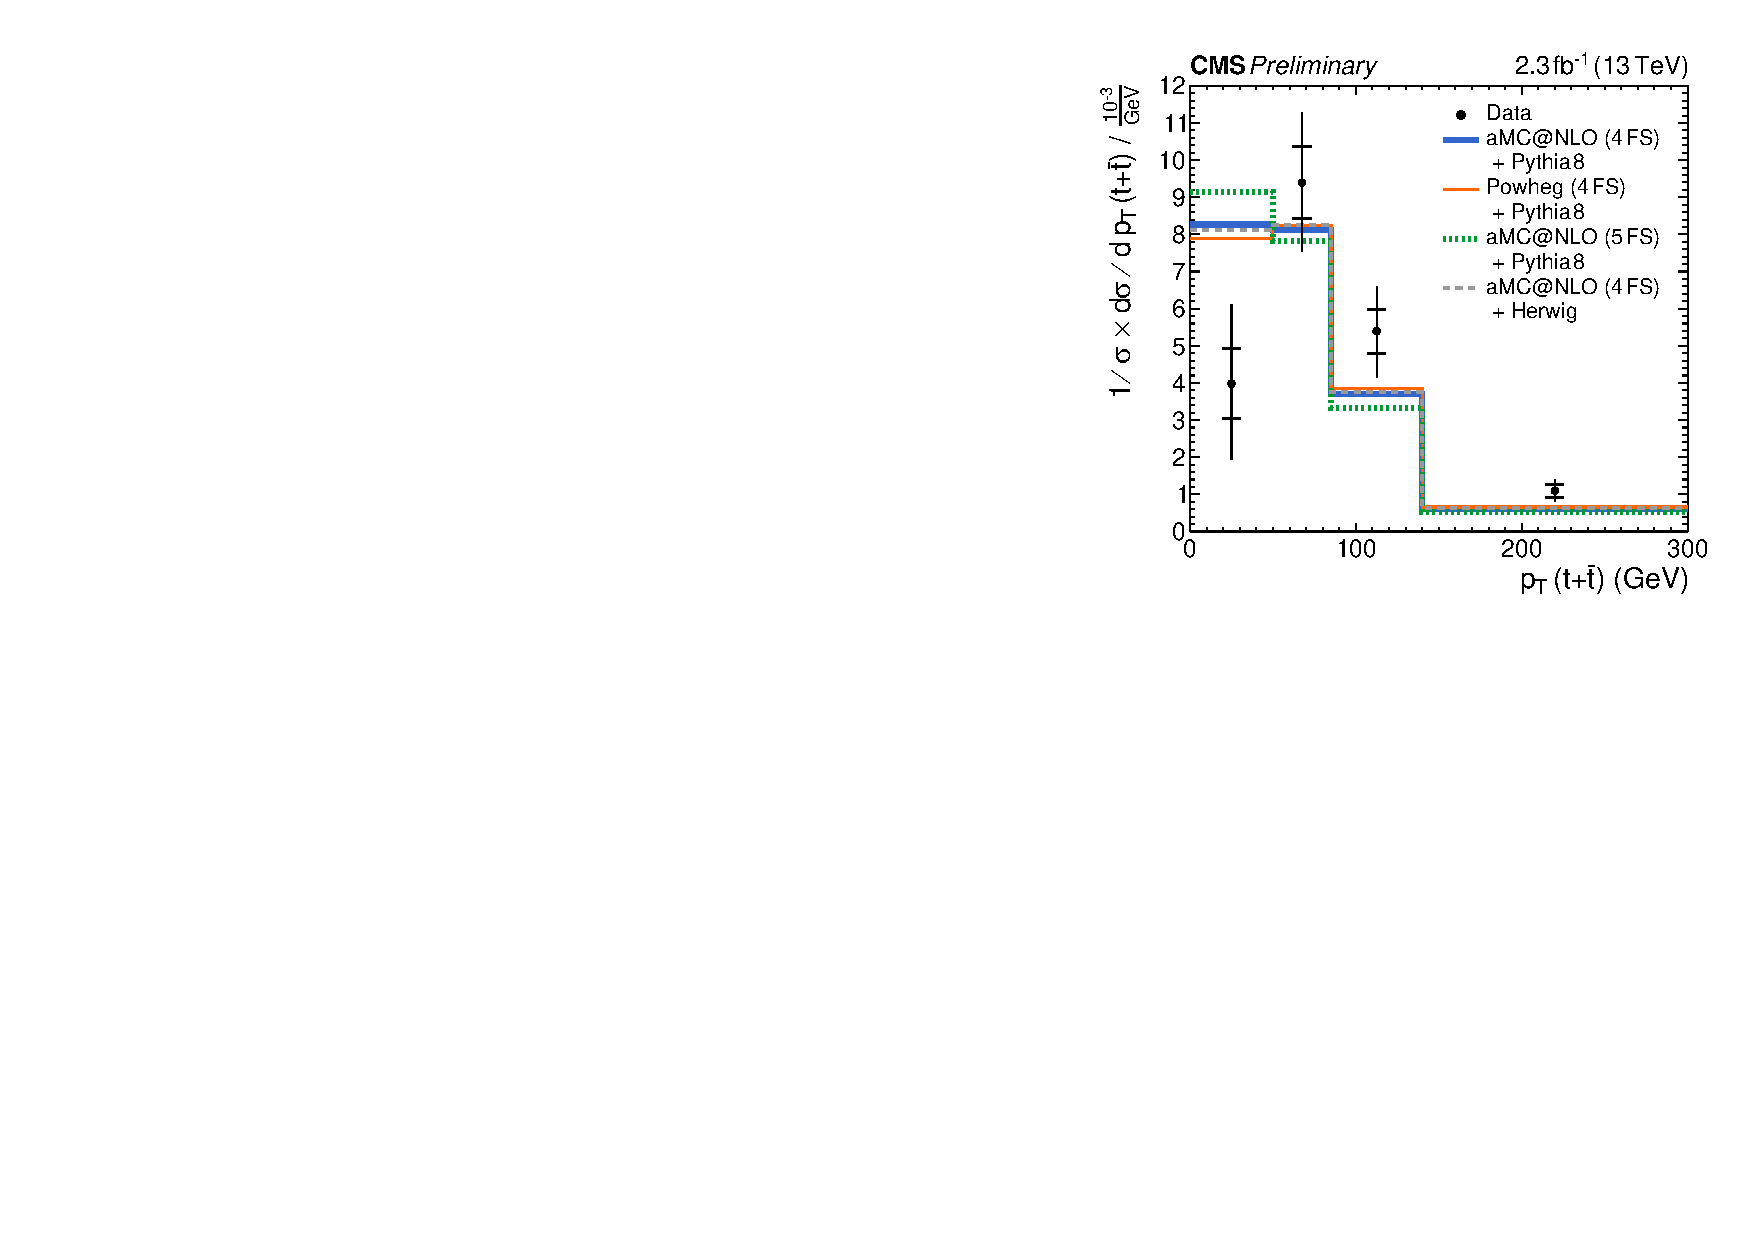
\includegraphics[width=0.45\textwidth]{figures/result/unfolded_top_pt.pdf}\hspace{0.05\textwidth}
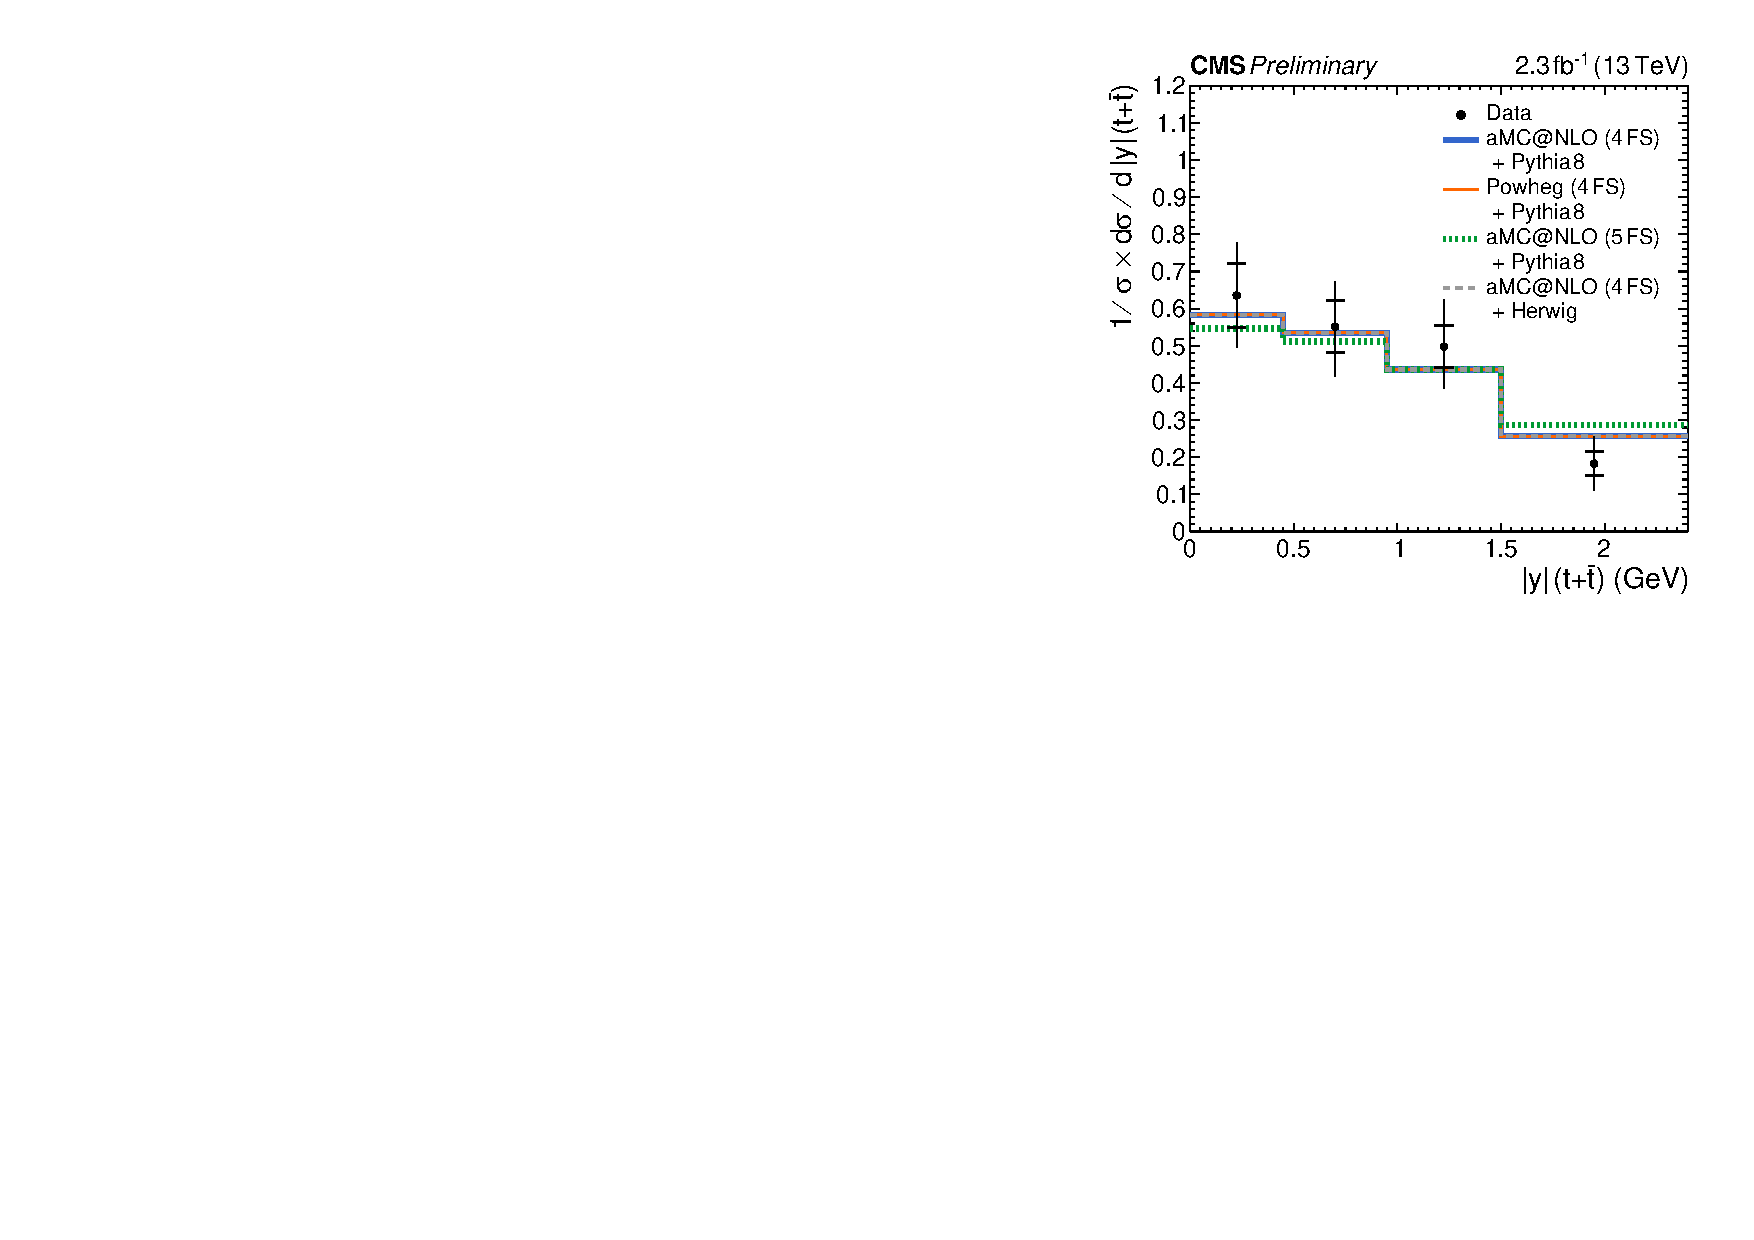
\includegraphics[width=0.45\textwidth]{figures/result/unfolded_top_y.pdf}
\end{center}

\caption{Normalized differential t-channel single-top-quark cross section as a function of the parton-level top quark (left)~transverse momentum and (right)~rapidity.}
\end{figure}



\section{Conclusion}





\begin{thebibliography}{99}

\bibitem{TOP-16-004} CMS Collaboration, \emph{CMS Physics Analysis Summary} CMS-TOP-16-004 (2016).
\bibitem{tunfold} S. Schmitt, \emph{JINST} \textbf{7} (2012) T10003.

\end{thebibliography}

 
\end{document}

